
\section{Experiment}
\subsection{Experimental Settings and Implementation Details}
We validate AdaSG over three typical image classification datasets, including \textbf{CIFAR-10}, \textbf{CIFAR-100} \cite{krizhevsky2009learning} and \textbf{ImageNet} (\textbf{ILSVRC2012}) \cite{russakovsky2015imagenet}. CIFAR-10 and CIFAR-100 contain 10 and 100 classes of images, respectively. Both of them are split into 50K training images and 10K testing images. ImageNet consists of 1.2M samples for training and 50k samples for validation with 1000 categories. For data-free setting, only validation sets are adopted to evaluate the performance of the quantized models.
In the experiments, we quantize pre-trained full-precision networks P including ResNet-20 for CIFAR, and ResNet-18, ResNet-50, and MobileNetV2 for ImageNet, via the following quantizer to yield the quantized networks Q:

\noindent \textbf{Quantizer.}
Following \cite{xu2020generative,choi2021qimera}, we quantize both full-precision (float32) weights and activations into $n$-bit precision via a symmetric linear quantization method based on \cite{jacob2018quantization} below:
\begin{small}
\begin{equation}
\theta_q=round \Big ((2^n-1) * \frac{\theta-\theta_{min}}{\theta_{max}-\theta_{min}}-2^{n-1} \Big),
\end{equation}
\end{small}
where $\theta$ and $\theta_q$ are the full-precision and quantized value. $round(\cdot)$ returns the nearest integer value to the input. $\theta_{min}$ and $\theta_{max}$ are the minimum and maximum of $\theta$, respectively.
Regarding the bit width $n$, we select 3-bit, 4-bit and 5-bit precision, which are representative for low-bit and high-bit cases, particularly: 3-bit quantization actually leads to a huge performance loss, which is a major challenge for the existing DFQ methods; while 5-bit or higher-bit quantization usually causes a small performance loss, which is selected to validate the generalization ability. 

For the \emph{maximization} process, we construct the architecture of the generator (G) following ACGAN \cite{odena2017conditional}, while P and Q play the role of discriminator, where G is trained with the loss function Eq.(\ref{generator_loss}) using Adam \cite{kingma2014adam} as an optimizer with a momentum of 0.9 and a learning rate of 1e-3.
For the \emph{minimization} process, Q is optimized with the loss function Eq. (\ref{calibration_loss}), where SGD with Nesterov \cite{nesterov1983method} is adopted as an optimizer with a momentum of 0.9 and weight decay of 1e-4. For CIFAR, the learning rate is initialized to 1e-4 and decayed by 0.1 for every 100 epochs, while it is 1e-5 (1e-4 for ResNet-50) and divided by 10 at epoch 350 (at epoch 200 and 300 for ResNet-50) on ImageNet. The generator and quantized model are totally trained for 400 epochs. The batch size is set to 16.
For the hyperparameters,  $\alpha$, $\beta$ and $\gamma$ in Eq.(\ref{generator_loss}); $\lambda_l$ and $\lambda_u$ in Eq.(\ref{boundary_loss}) are empirically set to be 0.1, 1, 1, 0.3 and 0.8. 
%(\emph{Due to page limitation, see our supplementary material for parameter studies}).
All experiments are implemented with pytorch \cite{paszke2019pytorch} based on the code of GDFQ \cite{xu2020generative} and run on an NVIDIA GeForce GTX 1080 Ti GPU and an Intel(R) Core(TM) i7-6950X CPU @ 3.00GHz.

To validate how AdaSG generates the sample with desirable adaptability to maximally benefit Q, we empirically validate why AdaSG works, including the comparisons with the  state-of-the-arts, ablation study as well as visual analysis.






\begin{table*}
\setlength{\abovecaptionskip}{0.02cm}
%\setlength{\belowcaptionskip}{-0.25cm}
\caption{Accuracy (\%) comparison with the state-of-the-arts on CIFAR-10, CIFAR-100 and ImageNet. $\dag$: the results implemented by author-provided code. -: no results are reported. \emph{n}w\emph{n}a indicates the weights and activations are quantized to \emph{n} bit. The best results are reported with \textbf{boldface}.}
\label{sota}
\centering
%\small
\scriptsize
%\tiny
%\footnotesize
\begin{tabular}{c|cc|c|  c| c| ccc  |c}
\toprule
\textbf{Dataset} &\tabincell{c}{\textbf{Model} \\ (Full precision)}     &\textbf{Bit width}  &\tabincell{c}{\textbf{ZAQ} \\ (CVPR 2021)} &\tabincell{c}{\textbf{IntraQ}  \\ (CVPR 2022)} &\tabincell{c}{\textbf{ARC+AIT}  \\ (CVPR 2022)}  &\tabincell{c}{\textbf{GDFQ} \\ (ECCV 2020)}    &\tabincell{c}{\textbf{ARC} \\ (IJCAI 2021)}    &\tabincell{c}{\textbf{Qimera} \\ (NeurIPS 2021)}    &\tabincell{c}{\textbf{AdaSG} \\ \textbf{(Ours)}}   \\
%\hline\hline
\bottomrule
\toprule
\multirow{3}{*}{\textbf{CIFAR-10}}
&                       &3w3a     &-      &77.07 &-  &\ 75.11$^{\dag}$     &-     &\ 74.43$^{\dag}$            &\textbf{84.14}   \\
&\emph{ResNet-20}      &\cellcolor{mygreen}4w4a     &\cellcolor{mygreen}92.13 &\cellcolor{mygreen}91.49 &\cellcolor{mygreen}90.49     &\cellcolor{mygreen}90.11     &\cellcolor{mygreen}88.55     &\cellcolor{mygreen}91.26    &\cellcolor{mygreen}\textbf{92.10}  \\
&(93.89)            &5w5a     &93.36 &-  &92.98   &93.38     &92.88     &93.46   &\textbf{93.76}   \\
%\hline\hline
\bottomrule
\toprule
\multirow{3}{*}{\textbf{CIFAR-100}}
&                       &3w3a     &-    &48.25 &-  &\ 47.61$^{\dag}$      &-    &\ 46.13$^{\dag}$           &\textbf{52.76}   \\
&\emph{ResNet-20}      &\cellcolor{mygreen}4w4a     &\cellcolor{mygreen}60.42 &\cellcolor{mygreen}64.98 &\cellcolor{mygreen}61.05    &\cellcolor{mygreen}63.75      &\cellcolor{mygreen}62.76    &\cellcolor{mygreen}65.10   &\cellcolor{mygreen}\textbf{66.42}  \\
&(70.33)            &5w5a     &68.70 &-  &68.40   &67.52      &68.40    &69.02   &\textbf{69.42}   \\

%\hline\hline
\bottomrule
\toprule
\multirow{3}{*}{\textbf{}}
&                       &3w3a    &-      &- &-  &\ 20.23$^{\dag}$   &23.37       &\ 1.17$^{\dag}$    &\textbf{37.04}   \\
&\emph{ResNet-18}      &\cellcolor{mygreen}4w4a    &\cellcolor{mygreen}52.64 &\cellcolor{mygreen}66.47 &\cellcolor{mygreen}65.73     &\cellcolor{mygreen}60.60   &\cellcolor{mygreen}61.32       &\cellcolor{mygreen}63.84    &\cellcolor{mygreen}\textbf{66.50}  \\
&(71.47)            &5w5a    &64.54 &69.94  &70.28    &68.49   &68.88       &69.29    &\textbf{70.29}   \\

\cline{2-10}
%\hline
\multirow{3}{*}{\textbf{ImageNet}}
&                       &3w3a    &-     &- &- &\ 1.46$^{\dag}$     &14.30    &-            &\textbf{26.90}   \\
&\emph{MobileNetV2}  &\cellcolor{mygreen}4w4a    &\cellcolor{mygreen}0.10  &\cellcolor{mygreen}65.10 &\cellcolor{mygreen}\textbf{66.47}   &\cellcolor{mygreen}59.43    &\cellcolor{mygreen}60.13    &\cellcolor{mygreen}61.62    &\cellcolor{mygreen}65.15  \\
&(73.03)           &5w5a    &62.35 &71.28 &\textbf{71.96}    &68.11   &68.40   &70.45    &{71.61}   \\

\cline{2-10}
%\hline
\multirow{3}{*}{\textbf{}}
&                       &3w3a      &-    &-  &- &\ 0.31$^{\dag}$      &1.63    &-            &\textbf{16.98}   \\
&\emph{ResNet-50}      &\cellcolor{mygreen}4w4a      &\cellcolor{mygreen}53.02  &\cellcolor{mygreen}-  &\cellcolor{mygreen}68.27 &\cellcolor{mygreen}54.16    &\cellcolor{mygreen}64.37   &\cellcolor{mygreen}66.25    &\cellcolor{mygreen}\textbf{68.58}  \\
&(77.73)            &5w5a      &73.38  &-  &76.00  &71.63    &74.13   &75.32    &\textbf{76.03}   \\
\bottomrule
\end{tabular}
\vspace{-0.8em}
\end{table*}









\subsection{Why does AdaSG Work?}
We experimentally verify the core idea of AdaSG --- generating the sample with desirable adaptability to recover the performance of Q with varied bit widths. We perform the data-free quantization experiments with ResNet-18 (3-bit and 5-bit precision) serving as both P and Q on ImageNet. 
Fig.\ref{ada_experiment}(a1)(b1) illustrates that the disagreement ($\mathcal{H}_{info}(p_{ds})$ in Eq.(\ref{metric})) between P and Q for AdaSG fluctuates stably within a small range compared to GDFQ \cite{xu2020generative} and Qimera \cite{choi2021qimera}, confirming that the generated sample with desirable adaptability by AdaSG is fully exploited to benefit Q, and the bound constraint loss (Eq.(\ref{boundary_loss})) can avoid generating the sample with too large or small adaptability, which leads to ridiculously large disagreement or agreement.
Fig.\ref{ada_experiment}(a2)(b2) reveals that the balance gap (Definition 3) keeps on par with zero (either BG $>0$ or BG $<0$) during the iteration process unlike GDFQ and Qimera, which confirm the principle that AdaSG achieves the stationarity of the DFQ game and the coordination between $\mathcal{L}_{ds}$ (Eq.(\ref{ds_ce})) and $\mathcal{L}_{as} $ (Eq.(\ref{las})) can generate the sample with desirable adaptability to maximally benefit Q.



\begin{figure}[t]
\centering
\setlength{\abovecaptionskip}{0.02cm}
\setlength{\belowcaptionskip}{-0.35cm}
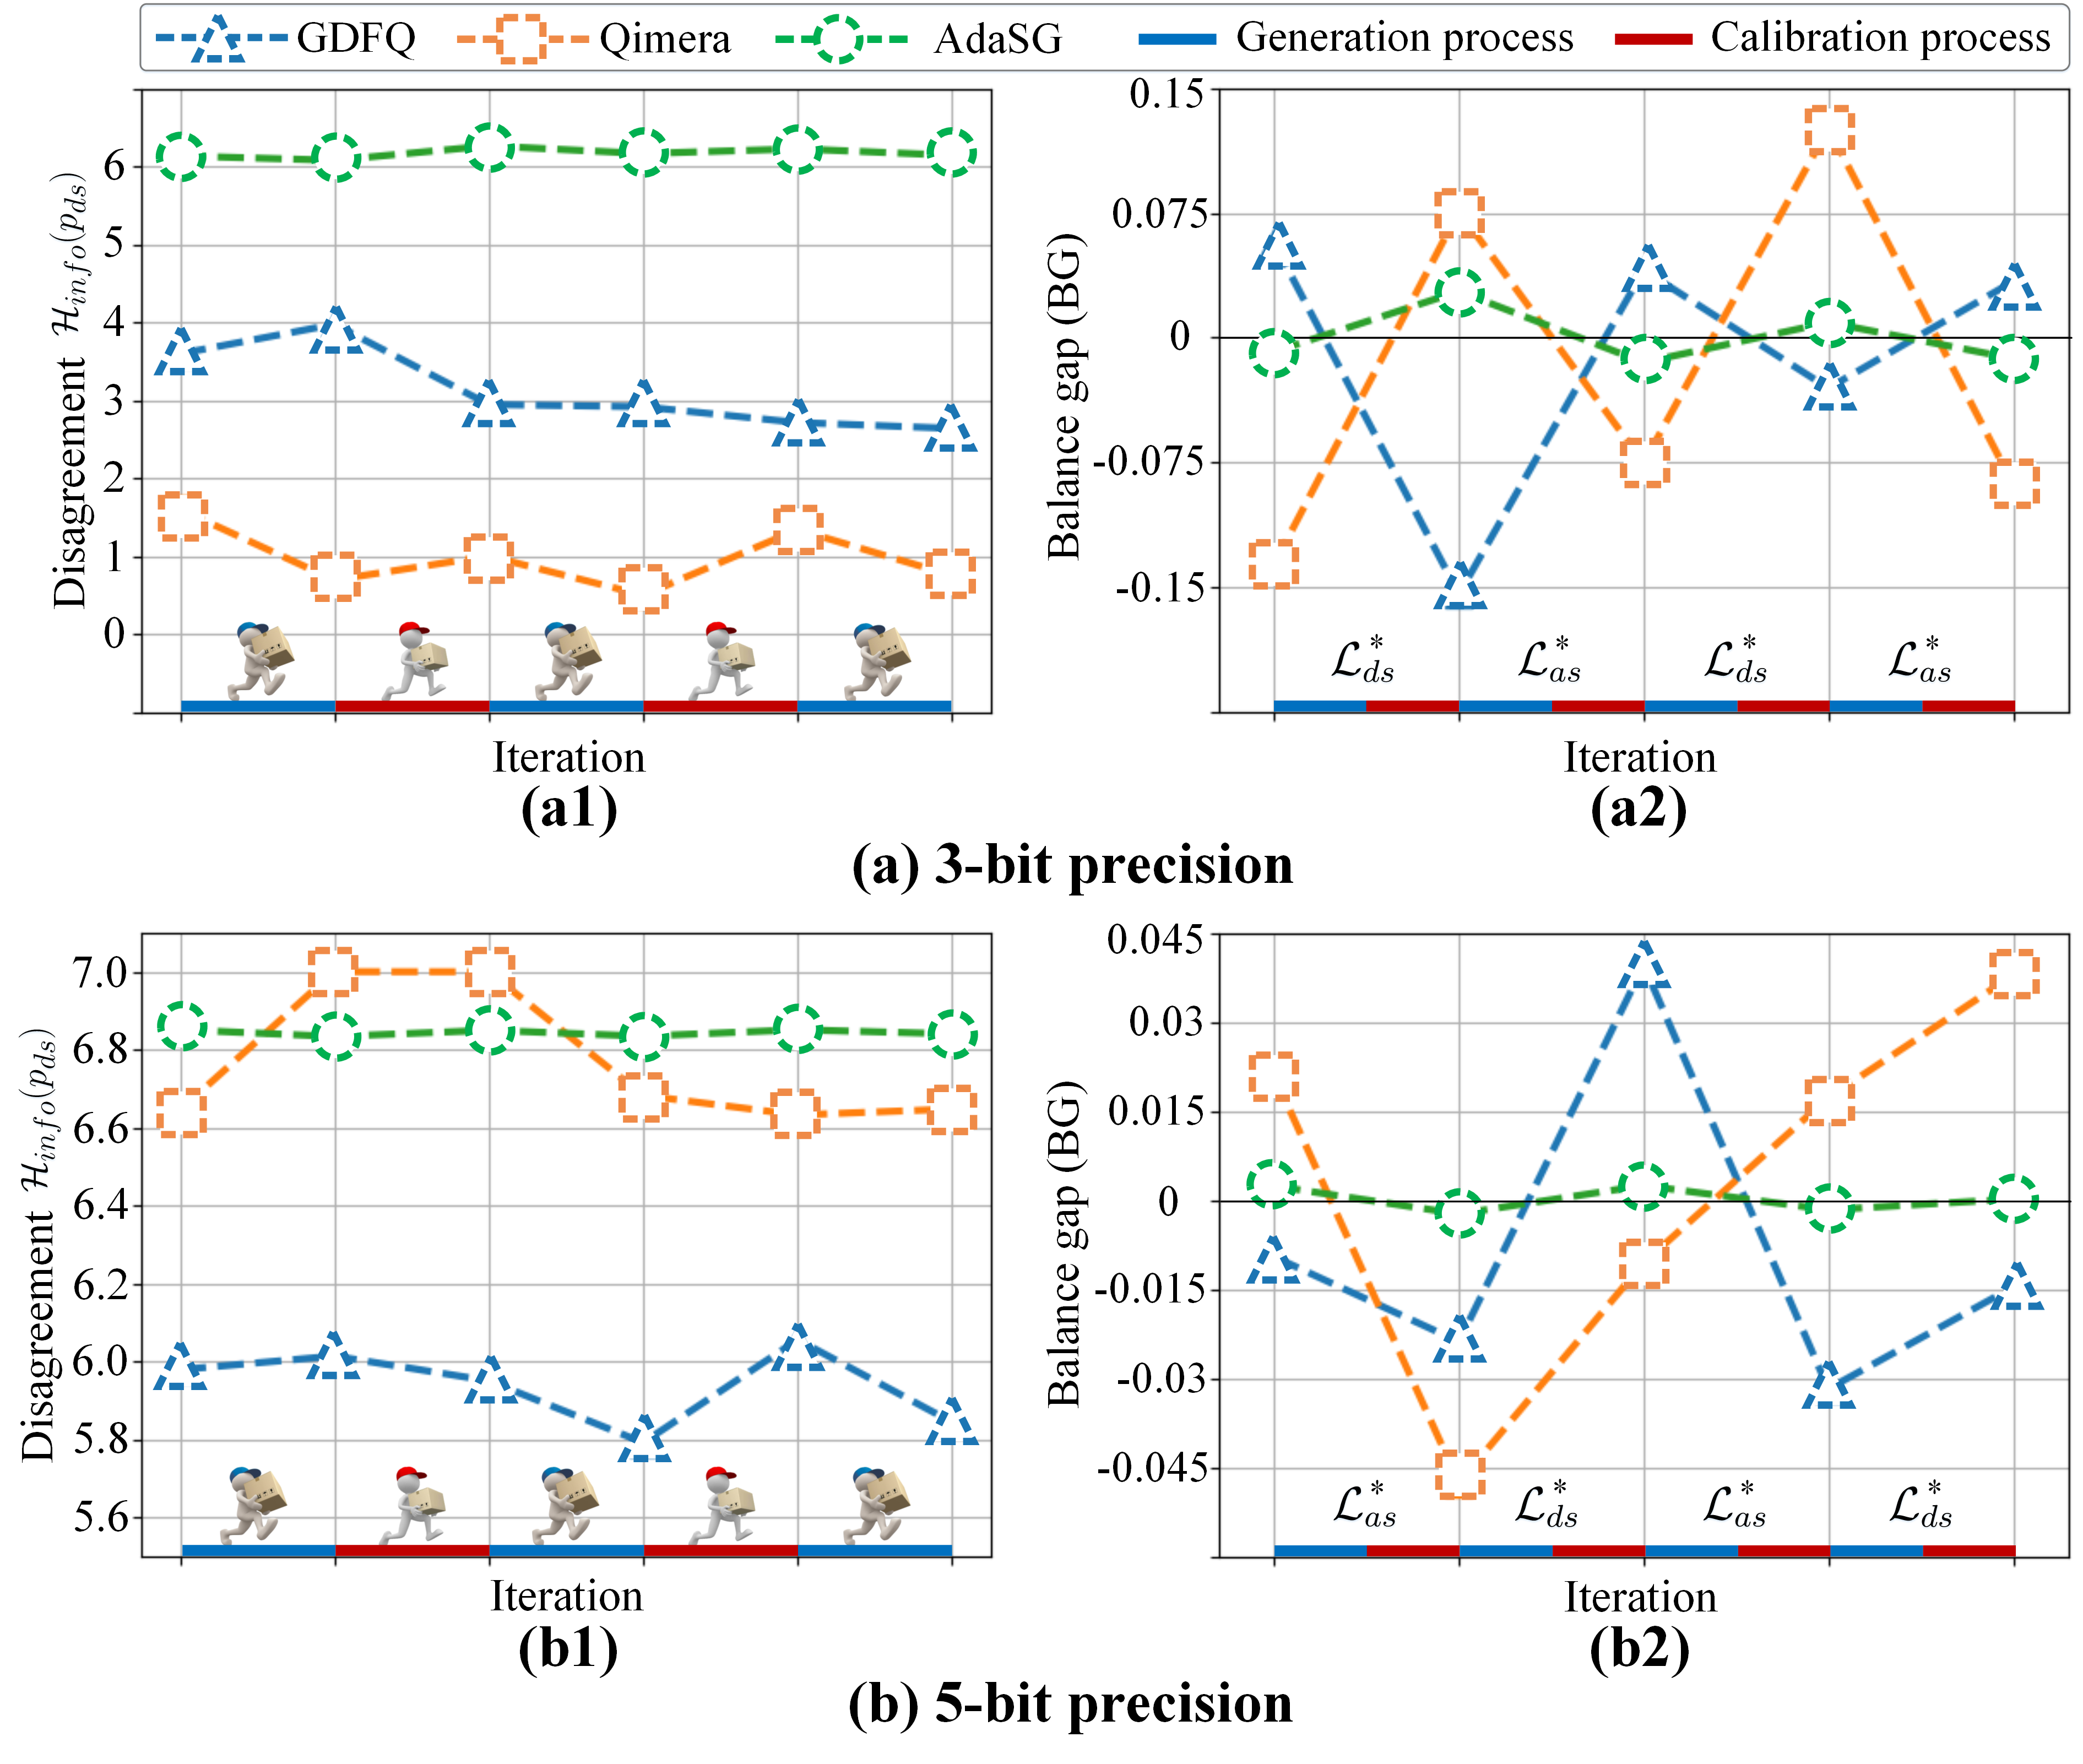
\includegraphics[width=1.0\columnwidth]{ada_experiment.png}
\caption{Illustration of AdaSG on generating the samples with desirable adaptability to Q under (a) 3-bit and (b) 5-bit precision. {(a1)(b1)} Disagreement (\emph{i.e.}, $\mathcal{H}_{info}(p_{ds})$) between P and Q during the generation (\textcolor[RGB]{0,112,192}{\textbf{---}}) and calibration (\textcolor[RGB]{192,0,0}{\textbf{---}}) process. (a2)(b2) Balance gap (BG).}
\label{ada_experiment}
\end{figure}








\begin{table}[t]
\setlength{\abovecaptionskip}{0.12cm}
\setlength{\belowcaptionskip}{-0.25cm}
\caption{Ablation study about varied components of AdaSG. \emph{n}w\emph{n}a indicates the weights and activations are quantized to \emph{n} bit. The best results are reported with \textbf{boldface}.}
\centering
\scriptsize
\begin{tabular}{c|c|c|c|c|c|c}
\toprule
%\tabincell{c}{\textbf{Model} \\ (Full precision)} &$\mathcal{L}_{ds}$ &$\mathcal{L}_{as}$     &$\mathcal{L}_b$  &$\mathcal{L}_{BNS}$    &3w3a  &5w5a   \\

\multirow{2}{*}{\tabincell{c}{\textbf{Model} \\ (Full precision)}} & \multirow{2}{*}{$\mathcal{L}_{ds}$} & \multirow{2}{*}{$\mathcal{L}_{as}$} & \multirow{2}{*}{$\mathcal{L}_b$} & \multirow{2}{*}{$\mathcal{L}_{BNS}$}  &\multicolumn{2}{c}{\textbf{Bit width}}  \\
\cline{6-7}
&&&&&3w3a &5w5a  \\

%\hline\hline
\bottomrule
\toprule
%\hline
\multirow{6}{*}{\tabincell{c}{\emph{ResNet-18} \\ (71.47)}}
&&\ding{51}      &\ding{51}           &\ding{51}                  &14.86     &69.15   \\
&\cellcolor{mygreen}\ding{51}&\cellcolor{mygreen}      &\cellcolor{mygreen}\ding{51}           &\cellcolor{mygreen}\ding{51}                  &\cellcolor{mygreen}26.41     &\cellcolor{mygreen}69.81  \\
&\ding{51}&\ding{51}      &           &\ding{51}                  &32.75     &70.13  \\
&\cellcolor{mygreen}&\cellcolor{mygreen}      &\cellcolor{mygreen}\ding{51}           &\cellcolor{mygreen}\ding{51}                                &\cellcolor{mygreen}15.01     &\cellcolor{mygreen}70.06   \\
&\ding{51}&\ding{51}      &\ding{51}           &                  &20.98     &67.35  \\
&\cellcolor{mygreen}\ding{51} &\cellcolor{mygreen}\ding{51}      &\cellcolor{mygreen}\ding{51}           &\cellcolor{mygreen}\ding{51}    &\cellcolor{mygreen}\textbf{37.04}     &\cellcolor{mygreen}\textbf{70.29}  \\

\bottomrule
\end{tabular}
\label{ablation}
\vspace{-2.4em}
\end{table}







\subsection{Comparison with State-of-the-arts}
To verify the superiority of AdaSG, we compare it with typical DFQ approaches, including: GDFQ \cite{xu2020generative}, ARC \cite{zhu2021autorecon} and Qimera \cite{choi2021qimera}: reconstructing the original data from P; ZAQ \cite{liu2021zero}  focuses primarily on the adversarial sample generation rather than adversarial game process for AdaSG; IntraQ \cite{zhong2022intraq} optimizes the noise to obtain fake sample without a generator; AIT \cite{choi2022s} focuses on improving the loss function and manipulating the gradients for ARC to generate better sample, denoted as ARC+AIT.

Table \ref{sota} summarizes our following observations: 1) AdaSG offers a significant and consistent performance gain over the state-of-the-arts, in line with our purpose of generating the sample with desirable adaptability to maximally benefit Q. Impressively, AdaSG achieves at most 9.71\%, 6.63\% and 35.87\% accuracy gains on CIFAR-10, CIFAR-100 and ImageNet, respectively. Especially, compared with GDFQ, ARC and Qimera where Q is independent of the generation process, AdaSG obtains accuracy improvement with a large margin, \emph{e.g.}, at least 0.3\% gain (ResNet-20 with 5w5a on CIFAR-10), confirming the necessity of AdaSG focusing on the sample adaptability to Q.   Specifically, ZAQ suffers from a large performance gap compared to AdaSG, since many unexpected samples are generated without considering the sample adaptability, which is harmful to calibrating Q.  AdaSG shows obvious advantages over AIT despite of the combination with ARC.
2) AdaSG achieves the substantial gains for Q with varied bit-widths, confirming the desirable adaptability of our generated sample to varied Q. Note that, for 3-bit case, most of the existing methods suffer from a poor accuracy, even fail to converge, while AdaSG obtains at most 35.87\% (ResNet-18 with 3w3a) and at least 4.21\% (ResNet-20 with 3w3a on CIFAR-100) performance gains.



\iffalse
\begin{table}[h]
\caption{}
\centering
\begin{tabular}{c|c|c|c|c|c}
\toprule
Dataset &Model     & Bit-width     &  GDFQ \cite{xu2020generative}    &Qimera \cite{choi2021qimera}  &\textbf{AdaSG}   \\
\hline\hline

\hline
\multirow{3}{*}{\textbf{CIFAR-10}}
&                       &3w3a           &75.11          &74.43$^{\dag}$            &\textbf{84.14}   \\
&ResNet-20      &4w4a           &90.11          &91.26    &\textbf{91.84}  \\
&(93.89)            &5w5a           &93.38          &93.46   &\textbf{93.48}   \\
\hline
\multirow{3}{*}{\textbf{CIFAR-100}}
&                       &3w3a           &47.61          &46.13$^{\dag}$           &\textbf{52.76}   \\
&ResNet-20      &4w4a           &63.75          &65.10   &\textbf{66.42}  \\
&(70.33)                       &5w5a           &67.52          &69.02   &\textbf{69.42}   \\
\bottomrule
\end{tabular}
\end{table}
\fi














\iffalse
\begin{figure}[h]
\centering
\includegraphics[width=0.8\textwidth]{entropy_dist.pdf}
\caption{}
\end{figure}
\fi



\subsection{Ablation Study}

\textbf{Validating adaptability with disagreement and agreement samples}
As aforementioned, the disagreement and agreement samples play a critical role on the sample adaptability to Q, which serve as a pivotal role between the maximization and minimization process during the zero-sum game. We conduct the ablation study on $\mathcal{L}_{ds}$ (Eq.(\ref{ds_ce})) and $\mathcal{L}_{as} $ (Eq.(\ref{las})) over ImageNet. Table \ref{ablation} suggests the great superiority (37.04\% and 70.29\%) of AdaSG (including the both) to other cases. It is worth noting that, removing either or both of $\mathcal{L}_{ds}$ and $\mathcal{L}_{as} $ obtains a large performance degradation (at most 22.18\% and 1.14\%), implying the intuition of the cooperation between $\mathcal{L}_{ds}$ and $\mathcal{L}_{as} $.
Interestingly, the case without $\mathcal{L}_b$ (Eq.(\ref{boundary_loss})) receives the minimal accuracy loss (4.29\% and 0.16\%), confirming the importance of $\mathcal{L}_b$ on the basis of $\mathcal{L}_{ds}$ and $\mathcal{L}_{as}$.










\subsection{Visualization of Generated Samples}
To further show the desirable adaptability of the generated samples by AdaSG to Q, we conduct the visual analysis over MobileNetV2 serving as both P and Q on ImageNet by the similarity matrix (each element is obtained by computing the $\ell_1$ norm between the probability distribution $p_{ds}$ of every two samples), along with the visualization of generated samples in Fig.\ref{simi-visual}. Fig.\ref{simi-visual}(a) illustrates that the generated samples by AdaSG possess a much larger similarity (the darker, the larger) than those by GDFQ, implying that the generated sample by GDFQ varies greatly, where a lots of samples with undesirable adaptability exist against AdaSG. Fig.\ref{simi-visual}(b) shows that the samples generated for 3-bit and 5-bit precision vary greatly, while the samples from varied categories also differ greatly from each other, verifying that the samples possess desirable adaptability to varied Q, upon the fact that the category (label) information is fully exploited.









\begin{figure}[t]
\centering
\setlength{\abovecaptionskip}{0.12cm}
\setlength{\belowcaptionskip}{-0.35cm}
\includegraphics[width=1.0\columnwidth]{simi-visual.pdf}
\caption{{(a)} The similarity comparison between the generated samples. {(b)} Visualization of the generated samples, where each row denotes one of 8 randomly chosen classes from ImageNet.}
\label{simi-visual}
\end{figure}

























